% v3, 4 November 2026. Author metadata is intentionally absent in this review copy.
\documentclass[pre,twocolumn,superscriptaddress,showpacs,floatfix]{revtex4-2}
\usepackage{amsmath,amssymb,bm,graphicx,xcolor}
\usepackage{xr-hyper}
\usepackage[colorlinks=true,linkcolor=blue!60!black,citecolor=blue!60!black,urlcolor=blue!60!black]{hyperref}
\newcommand{\qs}{q^{*}}
\newcommand{\ds}{\mathrm{d}}

\externaldocument[S-]{supplement}
\begin{document}
\title{Discontinuous transition into two symmetric absorbing states in two dimensions}
\date{4 November 2026}
\begin{abstract}
A magnetization jump at a transition into two symmetric absorbing states
does not by itself distinguish a discontinuous loss of activity from
generalized voter criticality. We study a short-range binary lattice model
combining the self-complementary Day \& Night rule, voter copying, and a
local minority flip. At voter weight $p=1/2$, bulk bond activity stays near
0.29 across the measured planar-front reversals, in systems up to
$16384^2$ sites followed for five million steps. About 21\% of sites
continue to flip per step. Independently prepared fronts change direction
in the same narrow parameter region; metastable bulk decay and opposing
growth of disks and holes provide complementary evidence for a
discontinuous active--absorbing transition. A wall between the two absorbing
phases accumulates an increasing amount of active material. Small
directional differences remain sensitive to geometry and inference, and
the wetting exponent is unresolved. Toward the voter point the invasion
scale is approximately $q^*\propto\alpha(1-p)$. A finite-time coalescing-walk
closure explains this scale and identifies terms capable of bistability,
but longer runs expose continuing relaxation near the endpoint and leave
its asymptotic transition order open.
\end{abstract}
\maketitle
\raggedbottom
\setlength{\parskip}{0pt}

\section{Introduction}
\label{sec:intro}

A transition into an absorbing state eliminates fluctuations. With two
symmetry-related absorbing configurations, it can also select one of two
ordered states. In two dimensions this combination is closely associated
with generalized voter (GV) criticality, whose interface density vanishes
logarithmically~\cite{dornic2001,clifford1973,holley1975,cox1986,krapivsky1992},
or with separate Ising symmetry breaking and directed-percolation
absorption~\cite{droz2003,alhammal2005,vazquez2008,azizi2020}.
A magnetization jump occurs even at a GV transition. Establishing a
discontinuous loss of activity therefore requires a local activity
measurement and evidence about phase competition.

The Langevin description of Al Hammal \emph{et al.} includes a bistable
deterministic drift, but their two-dimensional simulations gave a GV
transition, with preliminary first-order behavior reported in three
dimensions~\cite{alhammal2005}. Subsequent microscopic studies found GV
and Ising--DP scenarios~\cite{castellano2009,azizi2020}.
Rodrigues \emph{et al.} reported a discontinuous paramagnetic--absorbing
line on a triangular lattice using magnetization and susceptibility
measurements~\cite{rodrigues2015}. The question addressed here is narrower
than the first occurrence of a discontinuous line: can finite local activity,
coherent interfacial competition, and nucleation be measured together in a
two-dimensional binary model with exactly two absorbing configurations?

Discontinuous absorbing transitions are established in reaction
models~\cite{ziff1986,bidaux1989,lubeck2006}, in models with three symmetric
absorbing states~\cite{lipowski2002,azizi2018}, and in ecological models with
two competing absorbing alliances~\cite{szabo2004,guisoni2013}.
The alliances contain many configurations and retain internal dynamics;
their fronts and active boundary layers nevertheless provide close
precedents. Our construction uses binary sites and a flip table depending
only on the number of disagreeing neighbors. It belongs to the nonlinear
voter family~\cite{cox1991,molofsky1999,schweitzer2009}.
A positive voter component removes all frozen configurations except the
two uniform states.

We concentrate on $p=\alpha=1/2$. Bulk simulations resolve a dense active
branch across the measured reversal region of independently prepared
fronts. Decay below that region develops absorbing domains after a
long-lived active stage; a disk and a hole exchange their growth
directions on opposite sides. Front measurements at several orientations
test the possibility of orientation-dependent coexistence, which is allowed
out of equilibrium~\cite{wang2015,liu2018}, without assuming a unique
thermodynamic coexistence point. A wall between the two absorbing states
also develops a layer of active material.

The approach to the voter point is a separate question. We examine longer
runs that distinguish a persistent branch from a slowly decaying apparent
plateau. A finite-time voter closure, motivated by perturbation theory
in $d\ge3$~\cite{cox2013}, yields an invasion scale proportional to
$\alpha(1-p)$. Contributions with at least five distinct ancestral
lineages can generate bistability in that closure; matching it to the
two-dimensional stochastic process remains uncontrolled.
The five-cell rule of Molofsky \emph{et al.} supplies a useful comparison,
reported in the supplement: a small-seed growth crossover and the onset
of coherent expansion can be measured there, but a metastable retreating
active slab is not resolved. This distinction limits what the closure
can be said to explain.

\section{Model}
\label{sec:model}

\subsection{Definition}

Each site $i$ of an $L_x\times L_y$ square lattice with periodic boundaries carries a state
$\sigma_i\in\{0,1\}$. Let $j_i$ be the number of sites among the eight Moore neighbors of $i$
whose state differs from $\sigma_i$. In one time step every site is updated simultaneously and
flips with probability $w(j_i)$, independently of the others, where
\begin{equation}
w(j) = (1-p)\,\alpha\,R(j) + p\,\frac{j}{8} + q\,\delta_{j,2},
\label{eq:rule}
\end{equation}
with $R(j) = 1$ for $j\in\{3,6,7,8\}$ and $R(j) = 0$ otherwise. The first term is the D\&N rule
B3678/S34678: a dead site becomes alive if it has 3, 6, 7, or 8
live neighbors, and a live site survives if it has 3, 4, 6, 7, or 8. The rule is
self-complementary, so in terms of disagreeing neighbors a site flips if and only if
$j\in\{3,6,7,8\}$, whatever its state. With probability $\alpha$ a site applies this flip
($\alpha$-asynchronous updating~\cite{fates2005,blok1999}). The second term is the synchronous
voter model on the Moore neighborhood: with probability $p$ the site copies a randomly chosen
neighbor. Since $w$ depends on the configuration only through $j$, Eq.~\eqref{eq:rule} is a
synchronous nonlinear voter model~\cite{cox1991,molofsky1999,schweitzer2009} with a nonmonotone
rate. The third term is a minority flip: a site with exactly two disagreeing neighbors flips
with additional probability $q$. We fix $\alpha = 1/2$ unless stated otherwise and use $q$ as the
control parameter; $p$ interpolates between the D\&N and voter contributions.
The voter point itself is $(p,q)=(1,0)$.
The probability range is $0\le p,\alpha\le1$ and $0\le q\le1-p/4$;
all simulated points lie within it.

Since $w(0) = 0$, the uniform states (all 0, all 1) are absorbing, and Eq.~\eqref{eq:rule} is
invariant under $\sigma\to 1-\sigma$. At $p=\alpha=1/2$, the sampled lower-$q$ runs coarsen toward the
absorbing states. Larger-$q$ runs sustain a disordered active region with
finite interface density and magnetization near zero over the observed windows.

\begin{figure*}
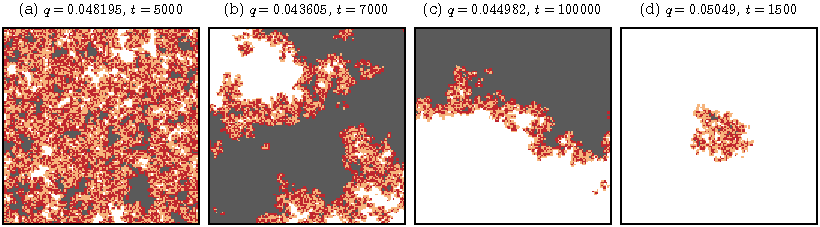
\includegraphics[width=\textwidth]{figs/fig_snap}
\caption{Configurations at $p = \alpha = 1/2$. Sites without a disagreeing Moore
neighbor are white (dead) or gray (alive); sites with at least one are orange (dead) or red
(alive). (a) The active phase, $q = 0.048195$, $t = 5000$, $L = 256$. (b) Decay of the metastable
active phase by nucleation and growth of the two absorbing phases, $q = 0.043605$, $t = 7000$
($256^2$ window of $L = 512$). (c) A wall between the two absorbing phases, wetted by a layer of the
active phase, $q = 0.044982$, $t = 10^5$. (d) A supercritical droplet, $q = 0.05049$, $t = 1500$,
grown from a disordered disk of radius 20.}
\label{fig:snap}
\end{figure*}

\subsection{Exactly two absorbing states}
\label{sec:lemma}

A configuration is absorbing when no site can flip, i.e., when $w(j_i) = 0$ for all $i$.

\textit{Lemma.} On the square lattice with the Moore neighborhood, every rule with $w(0)=0$ and $w(j)>0$ for
all $j\in\{3,\dots,8\}$ has exactly two absorbing configurations, the two uniform ones,
whatever the values of $w(1)$ and $w(2)$.

\textit{Proof.} A nonuniform configuration contains two nearest neighbors $x$ and $y$ (sharing an
edge) in different states. They disagree with each other, and they share four further Moore
neighbors, each of which disagrees with exactly one of them. Hence $j_x + j_y \ge 2 + 4 = 6$, so
$j_x\ge 3$ or $j_y\ge 3$, and that site flips with positive probability. $\square$

For $p>0$, Eq.~\eqref{eq:rule} gives $w(j)\ge pj/8>0$ for every $j\ge 1$, so the lemma applies.
For $0<p<1$ and $0<\alpha<1$ in the parameter range studied, $w(j)<1$ as well. Every configuration of a finite lattice then reaches consensus with
positive probability (by repeatedly flipping only the boundary sites of the live clusters), so
the two uniform states are the only recurrent ones.
At $p=0$, additional frozen configurations exist in exponentially large
number (Supplemental Sec.~\ref{S-app:frozen}); that directly simulated reference
lies outside the exactly-two-state regime. The representative point below
is nonmonotone; the conditions for attractiveness and the pair approximation
are given in Supplemental Secs.~\ref{S-sec:mf} and \ref{S-app:pa}.

\subsection{Observables}

We measure the density $\rho$ of disagreeing nearest-neighbor bonds (the interface density per
bond), the fraction $\iota$ of sites with at least one disagreeing Moore neighbor, and the
magnetization $m = 2n-1$, where $n$ is the fraction of live sites. In the active phase
$\rho\approx 0.2$--$0.4$ and $m$ fluctuates around zero; in either uniform
absorbing phase $\rho = \iota = 0$.
The bond density is our activity order parameter. If $a$ denotes the expected
fraction of sites flipping in one step, then
\begin{equation}
 a=\frac{1}{L^2}\sum_i w(j_i)\ge\frac{p}{8L^2}\sum_i j_i\ge\frac{p}{2}\rho .
 \label{eq:activitybound}
\end{equation}
The last inequality counts just the four axial neighbors. Thus, for $p>0$,
a positive bond density implies positive microscopic flip activity.

Since every finite lattice ultimately absorbs at the interior parameters,
the active branch refers to the order of limits
\begin{equation}
 \rho_{\rm act}(q)=\lim_{t\to\infty}\lim_{L\to\infty}
     \mathbb E_{1/2}[\rho_L(t;q)],
 \label{eq:limits}
\end{equation}
when this limit exists, starting from independent density-$1/2$ spins.
A discontinuity means a positive active-side limit on approaching a phase
boundary $q_c$. Our measurements are finite-volume, finite-time diagnostics
of that property. We denote a measured front crossing by $q^*$, with its
window and geometry stated; it need not be a unique limiting $q_c$.
At generalized voter criticality $\rho$ vanishes logarithmically, while a
magnetization jump can still occur~\cite{dornic2001,alhammal2005}.
We therefore compare density with coherent front reversal, metastable decay,
and the response to prepared droplets.

Spatial correlations use $s_i=2\sigma_i-1$ and the axis average
\begin{equation}
C(r)=\frac{1}{2L^2}\left\langle\sum_i s_i
\bigl(s_{i+r\hat x}+s_{i+r\hat y}\bigr)\right\rangle.
\label{eq:correlation}
\end{equation}
The random-start ensemble is exactly spin symmetric, so $\langle s_i\rangle=0$.
We retain the raw spin product, including $C(r)=1$ in absorbed configurations,
and do not subtract a separately estimated mean from each realization.

%=====================================================================================

\section{Methods}
\label{sec:methods}

We use independently seeded runs in five geometries: random density-$1/2$
bulk states, axial and tilted half-active bands, random active disks or
absorbing holes, small seeds in an absorbing background, and walls between
the two absorbing states. One step is one simultaneous lattice update.
The bit-parallel CPU simulator and dense CUDA backend use position- and
time-indexed Philox random numbers~\cite{salmon2011}. Their integer updates,
profiles and transferred checkpoints agree bit for bit in the archived
validation cases. The full protocols and computational checks are in
Supplemental Secs.~\ref{S-sec:protocols} and \ref{S-app:numerics}.

For the extended band measurements, a normal $(a,b)$ defines the coordinate
$s=(ay-bx)\bmod L$, with normal spacing $1/\sqrt{a^2+b^2}$.
We smooth over nine physical lattice spacings and follow the two exterior
profile crossings. Half the rate of change of their separation defines
the normal velocity. A complete declared cohort contributes to a window
only if every run retains the separated-front geometry throughout.
Interior activity is checked separately: the loss of a contour in a
dissolving band is not interpreted as coherent front retreat.

We integrate each bulk trajectory in time and weight independent runs
equally, including absorbed trajectories through their known absorbing
state. First recorded half-density loss and complete consensus are distinct
events; lifetime summaries retain censoring. Droplet growth means reaching
the finite box boundary before extinction and before the stated horizon,
not survival forever. Escapes are separately counted in seed experiments.

Independent runs, not lattice sites or output records, are the sampling
units. The large-system ensembles have four runs per point. Percentile
bootstrap intervals describe the observed run variation conditional on the
chosen estimator and window; with four runs their nominal $95\%$ level
does not ensure calibrated coverage. We display individual paired changes
for delicate drift claims and report small-sample reference calculations
separately. Geometry, fitting choices, finite size and finite time remain
systematic uncertainties rather than components of a pooled error bar.

\section{Phase competition at $p=\alpha=1/2$}
\label{sec:flagship}
\subsection{Front reversal and its resolution}
\label{sec:fronts}

At this representative point the bulk and interfacial evidence are best
resolved. Figure~\ref{fig:flagship} places the complementary observations
on their actual probability scales. In independently prepared strips the
active region retreats at lower $q$ and advances at higher $q$. Near
reversal, its interior retains substantial activity: the fronts bound an
active phase rather than a fragmenting remnant.

The late axial crossing in the independent $10^7$-step cohort is
$q^*=0.04594117$ over $5$--$10\times10^6$ steps. Slopes of integrated bond
activity, interface-site count, and live mass instead locate zeros at
0.04594075, 0.04594075, and 0.04594063. These are different estimators of
the same trajectories; their agreement checks the threshold definition
without adding independent realizations.
The crossing shifts from 0.04593717 in the earlier $2$--$5\times10^6$
window. The threshold-based shift remains positive in a small-sample reference
calculation, whereas the integrated bond-activity shift is smaller and
its interval includes zero (Supplemental Sec.~\ref{S-sec:sfronts}).
The remaining time dependence is therefore estimator-dependent in this
small ensemble; it does not specify an extrapolation law.

For normal directions $(1,0)$, $(2,1)$ and $(1,1)$, crossings lie in the
same narrow probability region. The $L=16384$, $1$--$2\times10^6$ data
give an axial-minus-tilted difference of $4.66\times10^{-6}$ with the
threshold envelope, reduced to $2.70\times10^{-6}$ using integrated bond
activity. The statistical significance depends on the interval method;
the tilted bands also have different physical widths and interface
lengths at fixed $L$. We report these as small finite-geometry contrasts,
not a resolved limiting anisotropy.

We use $q^*=0.04594$ as a rounded operational reference and vary it over
$[0.04592,0.04596]$ for normalization sensitivity. This range encompasses
the available extended-front estimates. It is neither a confidence
interval for a limiting boundary $q_c$ nor a bound on later relaxation.
The detailed orientation and window comparisons are in Supplemental
Sec.~\ref{S-sec:sfronts}.

\begin{figure*}
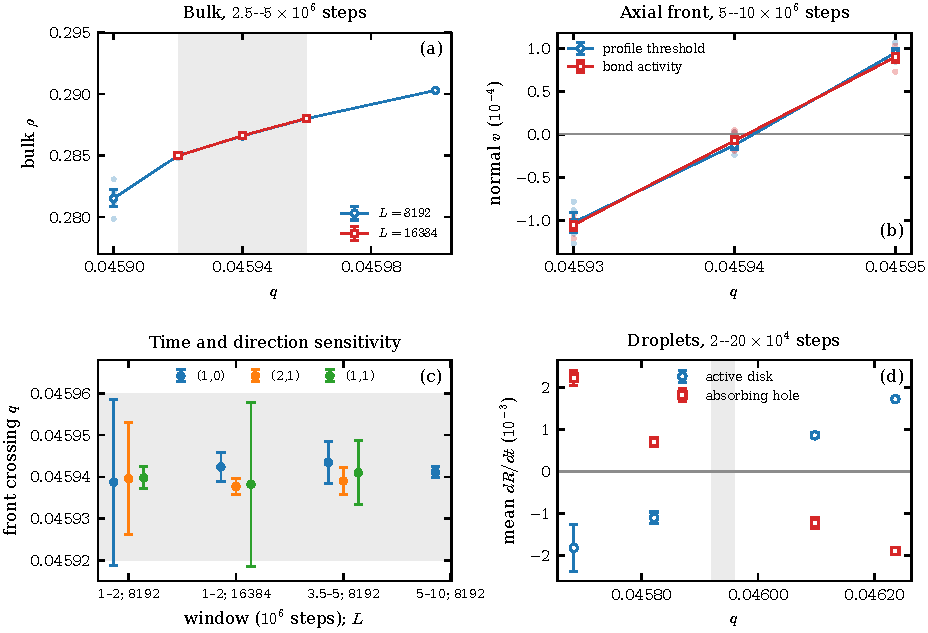
\includegraphics[width=\textwidth]{figs/fig_flagship}
\caption{Bulk and interfacial evidence at $p=\alpha=1/2$, plotted at the actual
probabilities $q$. (a) Unconditional bulk interface density, integrated over
$2.5$--$5\times10^6$ steps separately for each run, at $L=8192$ and 16384.
(b) Axial-front velocities for the independent $L=8192$, $T=10^7$ cohort,
fitted over $5$--$10\times10^6$. The profile-envelope estimate is compared
with the slope of the integrated bond activity, converted to an equivalent
width using the fixed reference density 0.2866. Four independent runs
contribute at every point in (a,b); faint symbols show individual runs and
bars give one standard error. Lines join group means.
(c) Envelope crossing estimates for the stated time windows and sizes.
The $T=2\times10^6$, $5\times10^6$, and $10^7$ cohorts are independent.
Bars are approximate pointwise delta-method Student-$t$ sensitivity intervals
with Welch--Satterthwaite degrees of freedom, conditional on the observed
bracketing pair. Small-sample coverage and bracketing uncertainty remain
limitations. All four runs must retain separated-front geometry throughout
the fit window; no invalid individual run is selectively removed.
(d) Growth rates of an active disk and an absorbing hole of initial radius
1000 on an $L=4096$ lattice, fitted over $2\times10^4$--$2\times10^5$ steps.
Bars are one standard error over four runs. The gray region in (a,c,d) is
the operational reference range $[0.04592,0.04596]$, used for normalization
sensitivity. It is not a confidence interval or an asymptotic bound.
The coarse droplet points in (d) do not resolve the smaller separations
between the front crossings in (c).}
\label{fig:flagship}
\end{figure*}


\subsection{A persistent dynamically active bulk}
\label{sec:bulk}

At $q=0.04594$, all four random-start $L=8192$ runs remain active through
$5\times10^6$ steps, with time-weighted mean $\rho=0.28659$ over the
last half. At $L=16384$, the corresponding four-run mean is 0.28661.
The means at the nearby $q=0.04592$ and 0.04596 are 0.28498 and 0.28803;
none of these twelve largest-system runs absorbs. Their late-window
density changes show no consistent decrease across the cohorts.
At the central probability, the actual fraction of sites flipping per
step has late mean 0.20874. The measured branch therefore retains
microscopic activity, independently of the bound in
Eq.~\eqref{eq:activitybound}.

The final configurations supply a spatial check.
At $q=0.04594$, $C(128)\simeq0.0046$ at both $L=8192$ and 16384;
the largest-system correlation drops from 0.427 at one spacing to
$5.7\times10^{-4}$ at $r=256$, with signed fluctuations about zero at
longer separations. The magnetic second-moment ratios on doubling size
are near one in a common late window (Supplemental Sec.~\ref{S-sec:sbulk}).
These are finite-scale checks at the sampled probabilities, not a
correlation-length extrapolation or an exclusion of every possible
intermediate critical regime.

On the lower-$q$ side the bulk exhibits delayed collapse accompanied by
the growth of absorbing domains [Fig.~\ref{fig:snap}(b)]. At
$q=0.045441$, for example, the mean time of recorded half-density loss
approaches $6.7\times10^4$ steps at the largest sampled sizes,
consistent with many droplets nucleating and growing locally.
Absorbing domains of opposite type leave active walls between them, so
half-density loss occurs before consensus.
On the active side, finite-volume survival instead increases strongly
with size. In independent $10^7$-step cohorts at $q=0.046359$, consensus
counts are $(32,32,6,0)$ out of 32 at $L=(64,128,192,256)$; at
$q=0.04605$ they are $(15,6,0)$ out of 16 at $L=(192,256,384)$ through
$3\times10^6$ steps. These size contrasts support a stable active branch
on the observed scales, but do not determine an asymptotic lifetime law.

\subsection{Opposing invasion and finite droplets}
\label{sec:opposing}

A disordered disk of radius $1000$ in the dead phase and a dead hole of
the same radius in an active background exchange growth directions
across the reversal region. All 32 trajectories, four for each geometry
at four probabilities, have the reported sign. The nearest sampled probabilities on opposite sides of reversal are 0.0458221 and 0.0460979; their separation,
$2.758\times10^{-4}$, is much wider than the directional crossing
differences. These measurements establish opposite invasion on the
sampled flanks. Radius traces and the curvature-law comparison are in
Supplemental Fig.~\ref{S-fig:drop2}.

They do not resolve an orientation-dependent coexistence interval.
Even for one isotropic zero, the model
$\ds R/\ds t=\pm v-D/R$ predicts shrinkage of both finite droplets
when $|v|<D/R$. With $D\simeq0.20$, $R=1000$ and the local axial
slope $\ds v/\ds q\simeq10.75$, this curvature-only full width is
about $3.7\times10^{-5}$ in $q$. Inferring generic coexistence from
droplet shrinkage would require sampling the candidate interval and
increasing the radius~\cite{wang2015,liu2018}.
Together, the finite bulk density, coherent invasion, and delayed
nucleation-driven decay provide the numerical case for a discontinuous
transition here. The precision of a unique limiting boundary is a
separate question.

\subsection{Critical droplets}
\label{sec:drops}

On the sampled active side, a small active region usually disappears:
the probability of growth increases with its initial size. We placed a disordered disk of radius $R$
(sites alive with probability $1/2$) in the dead state and ran 500--1000 independent replicas per
$(q,R)$ until extinction, boundary escape, or the declared time horizon
(Fig.~\ref{fig:drop}). All replicas in the completed disordered-disk ensembles resolve
to extinction or escape. The macroscopic-growth probability $P_{\rm grow}$
rises from 0 to 1 over a factor of about 3 in $R$, and the radius at which it reaches
$1/2$ grows as $q\to\qs$: $R_c = 2.6$, 4.8, 7.9, 12.5, 21, and 42 at $q/\qs = 2.0$, 1.40,
1.20, 1.10, 1.05, and 1.02. Plotted against the inverse planar-front velocity at the same $q$,
$R_c$ is approximately linear [Fig.~\ref{fig:drop}(b)], $R_c\simeq D/v + \Delta R$ with $D = 0.207$ and an offset
$\Delta R = 1.4$ sites, consistent with relaxation of the random initial disk; equivalently,
$R_c v = 0.21$--$0.26$ over a factor of 11 in $v$. The deterministic growth
law $\ds R/\ds t = v-D/R$ has curvature radius $D/v$; the fitted initial
radius includes the offset $\Delta R$. Curvature slows a convex active
region. In this
description, linear front reversal predicts $R_c\propto1/(q-\qs)$ near
coexistence; the finite-time measurements support the relation to $1/v$ over
the sampled range. Joint resampling of the binomial droplet outcomes and
independent front runs gives a conditional 95\% interval $D\in[0.182,0.230]$;
changing the front threshold and fit start gives $D=0.199$--$0.212$.
A $2\times2$ block of live sites, the standard initial
condition of spreading experiments, is far below $R_c$: it reaches the boundary with probability
$0.042\pm0.003$ at $q = 1.4\,\qs$ and $0.20\pm0.01$ at $2\,\qs$, and with probability $0.011$ at
$1.2\,\qs$ and $0.003$ at $1.1\,\qs$ (4000 replicas each), although the active phase is the stable
one there; the $R = 0.75$ disks of Fig.~\ref{fig:drop}(a), $2\times2$ blocks in which each site is
alive with probability $1/2$, reach it with probability $0.014$ and $0.061$ at
$1.4\,\qs$ and $2\,\qs$.
Here $R_c$ is the radius at which $P_{\rm grow}=1/2$ for the specified box
and observation horizon, not a strict minimum size or an infinite-time
survival threshold. Smaller seeds have a nonzero chance to grow. The useful
nucleation diagnostic is the increase of this probabilistic radius and its
relation to the independently measured front velocity.

\begin{figure*}
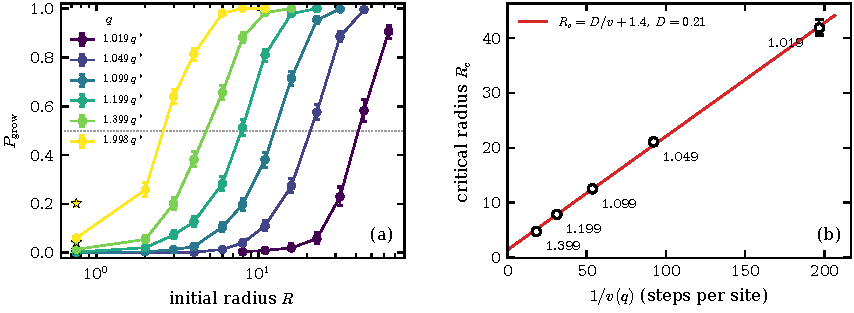
\includegraphics[width=\textwidth]{figs/fig_drop}
\caption{Critical droplets at $p = 1/2$. (a) Probability $P_{\rm grow}$ that a disordered disk of radius $R$
in the dead state reaches the lattice boundary before extinction and before
the declared time horizon, for $q/\qs$ from 1.02 to 2
(500--1000 replicas per point; at $R = 0.75$, a
$2\times2$ block with each site alive with probability $1/2$, 4000 replicas). Stars: the full
$2\times2$ block of live sites (4000 replicas). (b) Radius $R_c$ at
which $P_{\rm grow}=1/2$ against the inverse velocity of a planar front at the same $q$; labels
give $q/\qs$. The line is $R_c=D/v+\Delta R$. Disk protocols use
$L=512$--1024 and horizons $2\times10^4$--$3\times10^5$ depending on $q$;
the $2\times2$ block protocols use $L=1024$, $T=3\times10^4$.
Bars in (a) are 95\% binomial intervals from complete fixed-size replica
ensembles; vertical bars in (b) are conditional bootstrap intervals for the
interpolated $R_c$. The velocities use the corrected outer-envelope tracker.}
\label{fig:drop}
\end{figure*}


\subsection{Active material at a wall between absorbing phases}
\label{sec:wall}

A wall separating the all-alive and all-dead phases creates an active
layer without preparing an active region initially. We measure the
interface sites per unit wall length, $I=L_y\iota/2$, and subtract the
matched $q=0$ baseline to obtain excess adsorption $\Gamma=I-I_0$.
At $L_y=8192$, $L_x=16384$, four runs per point give
$\Gamma=133.27$, 166.15 and 190.86 at $q=0.04584$, 0.04588 and
0.04590 over $5$--$10\times10^6$ steps
(Fig.~\ref{fig:gpu_wetting}). The shorter walls, $L_x=4096$, give
134.80, 168.37 and 199.90. The closest point therefore retains a size
effect of about 4.5\%; each of the four longer-wall runs also declines
slightly between halves of the late window.

\begin{figure*}
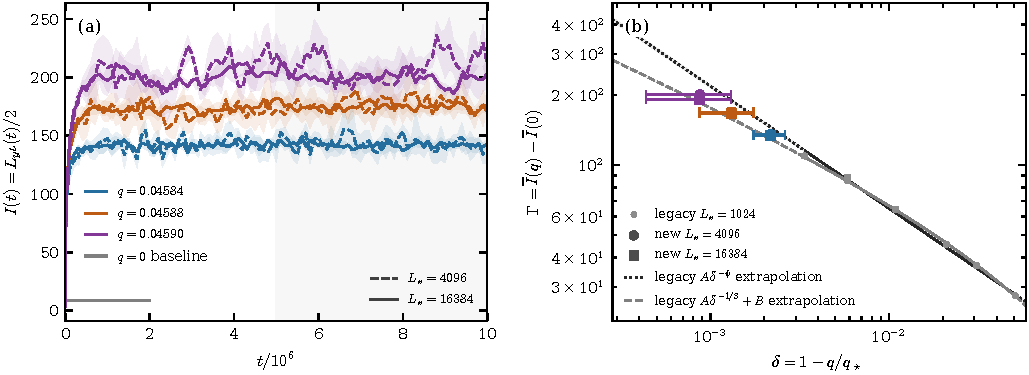
\includegraphics[width=\textwidth]{figs/fig_gpu_wetting}
\caption{Extended wall trajectories at $p=\alpha=1/2$, $L_y=8192$,
and $L_x=4096$ or 16384. Each nonzero-$q$ group contains four independent
runs to $10^7$ steps; each matching $q=0$ baseline contains two runs to
$2\times10^6$. (a) Interface sites per unit wall length. Line styles
distinguish $L_x$, and shading gives pointwise 95\% run-bootstrap
intervals. The gray span marks the $5$--$10\times10^6$ averaging window.
(b) Excess adsorption relative to the matched baseline. Vertical
intervals include shared-baseline sampling uncertainty; horizontal bars
show coexistence-reference sensitivity. Gray points and both
two-parameter fits use only the seven earlier $L_x=1024$ points.
Dashed and dotted continuations are predictions for the new data, with
conditional parameter-bootstrap bands at $q^*=0.04594$. These bands
exclude reference sensitivity and size/time systematics. No exponent is
fitted to the new data.}
\label{fig:gpu_wetting}
\end{figure*}


Increasing adsorption is consistent with a thickening active film, but
also depends on the activity inside the film. The existing measurements
establish neither divergence of the edge separation nor a wetting
exponent. Two-parameter fits to the earlier seven-point data, a pure
power and a one-third power with an additive offset, do not jointly
describe the new points within their sampling errors. Size, time,
and front-reference sensitivity remain visible
(Supplemental Sec.~\ref{S-sec:swall}).
Equilibrium complete wetting in two dimensions supplies a useful
comparison~\cite{lipowsky1983,fisher1984,carlon1999}, and active boundary
layers also occur between defensive alliances~\cite{szabo2007}.
Here a theory must describe the interaction of two fluctuating
active--absorbing fronts.

\section{The invasion scale and the voter endpoint}
\label{sec:line}
\subsection{Parameter survey}
\label{sec:phase}

The earlier strip survey gives a nonmonotonic invasion scale
(Fig.~\ref{fig:phase}; Supplemental Table~\ref{S-tab:line}). Starting
from the exceptional $p=0$ reference, it reaches a maximum near
$p=0.25$--0.5 and decreases toward $(p,q)=(1,0)$.
Over the sampled near-voter range it is approximately
$q^*\simeq0.25\alpha(1-p)$. The $p=0$ model has extra frozen states,
so that datum is not a measured $p\to0^+$ limit.
The survey densities were measured at specified probabilities and
observation windows; they are not extrapolated jumps.
In particular, the historical $p=0.99$ and 0.995 points are marked
separately in the figure. At the latter point, longer runs overturn
the apparent stationarity.

\begin{figure}
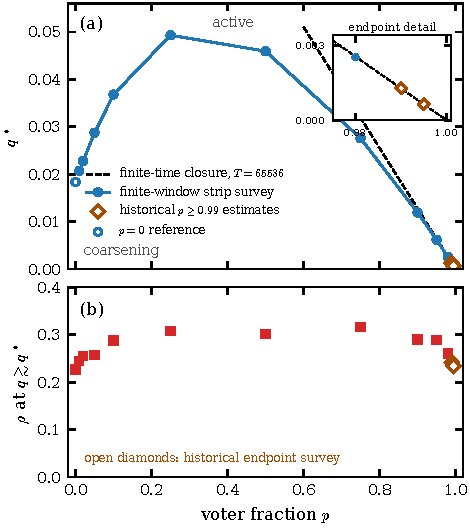
\includegraphics[width=\columnwidth]{figs/fig_phase}
\caption{(a) Finite-window invasion survey at $\alpha=1/2$ from strip
fronts (Table~\ref{S-tab:line}), with the refined $p=1/2$ operational
reference. The open blue circle denotes the $p=0$ reference with
additional frozen states. Open orange diamonds identify the historical
$p=0.99$ and 0.995 estimates; the inset enlarges the endpoint region.
The dashed line is the finite-time closure
$q_f(T)=c_f(T)\alpha(1-p)$ at $T=65536$, where $c_f=0.2553$.
(b) Time-weighted density at the actual nearby probabilities $q_\rho$
in Table~\ref{S-tab:line}, with equal run weights and one standard error.
Open orange diamonds again mark the historical endpoint survey.
The $p\ge0.99$ summaries combine nearby probabilities and observation
horizons. Longer trajectories at $p=0.995$, $q=0.000640$ show substantial
late decay in Fig.~\ref{fig:gpu_near20m}; the historical endpoint markers
do not locate a limiting transition or its density jump.}
\label{fig:phase}
\end{figure}


\subsection{Longer times reveal continuing relaxation}
\label{sec:voter}

At $p=0.995$, $q=0.000640$, four $L=8192$ trajectories run to
$2\times10^7$ steps have unconditional mean density 0.189 over
$5$--$10\times10^6$ and 0.122 over $10$--$20\times10^6$; one reaches
consensus. At $q=0.000642$ all four remain active, with late mean 0.2204,
but their paired changes between the two halves of the last window are
$-0.00154$, $-0.00578$, $-0.00155$, and $-0.00971$.
The mean change is $-0.00464$. Its percentile-bootstrap interval is
$[-0.0077,-0.0015]$, whereas a normal-reference paired $t_3$ interval
is $[-0.0109,+0.0016]$. The common sign is an observation about these
four runs; it is not a method-independent precision statement about
the population mean drift.
At $q=0.000644$ and 0.000648, the late means are 0.2265 and 0.2326,
with no consistent drift resolved over the same window.

\begin{figure*}
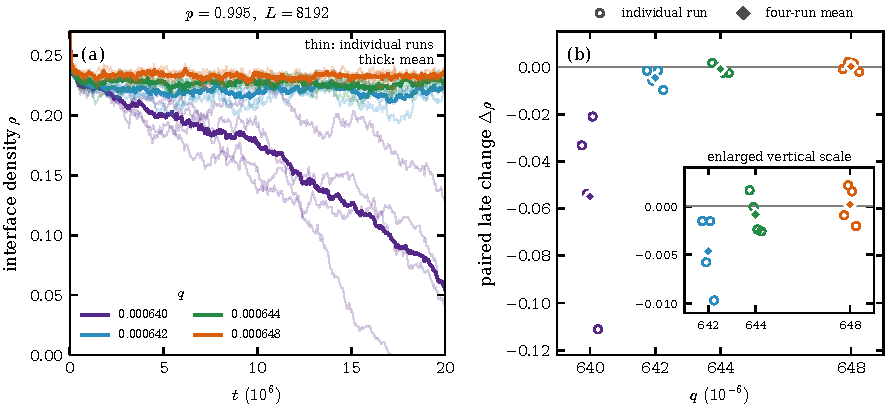
\includegraphics[width=\textwidth]{figs/fig_gpu_near20m}
\caption{Largest-system time dependence near the voter point,
$p=0.995$, $\alpha=1/2$, and $L=8192$. All four declared independent
runs at each $q=0.000640$, 0.000642, 0.000644, and 0.000648 are followed
to $T=2\times10^7$. (a) Thin curves show the individual trajectories
and thick curves their equal-run means. The trajectory that reaches
consensus at $q=0.000640$ contributes its known zero activity thereafter.
(b) Open circles show each run's time-weighted mean density over
$15$--$20\times10^6$ minus that over $10$--$15\times10^6$; diamonds
show the four-run means. Horizontal offsets separate the four runs
visually. The inset repeats the three higher-$q$ groups on an enlarged
vertical scale. The midpoint cohort at $q=0.000642$ was declared
independently after the original grid. The displayed run variation
does not assign a calibrated confidence level or establish stationarity.}
\label{fig:gpu_near20m}
\end{figure*}


The fronts reinforce the distinction between persistence and a measured
coexistence boundary. At $q=0.000640$ the strip interior decays strongly,
and only one of four runs keeps separated-front geometry over
$5$--$10\times10^6$ steps. Fitting its envelope would conflate invasion
with internal loss of activity. The higher-$q$ bands retain activity but
can encounter the finite box. These data do not locate a late stationary
front at the smallest probabilities (Supplemental Sec.~\ref{S-sec:svoter}).

Small seeds provide another finite-time diagnostic. At $p=0.99$,
$q=0.0012954$, a separately declared ensemble of eight million seeds
has 19 survivors and no boundary escapes at $t=10^6$. Counts fall from
793 to 97 between $t=63096$ and 251189, giving an effective survival
exponent of 1.52; the last sufficiently populated factor-four window
gives 1.26 with an interval including one. This quantifies strong
transient suppression at a specified probability.
A nonlinear voter model need not obey a voter asymptote before its
crossover~\cite{castellano2012,azizi2020}; the seed experiment therefore
does not locate criticality or establish survival at infinite time.
Magnetic size ratios and active-wall observations are also restricted
to their sampled points. None excludes an unsampled Ising--DP interval.

Reducing each site's update probability to $r=1/2,1/4,1/8$ changes
the measured invasion scale while retaining finite-time active and
front signatures (Supplemental Sec.~\ref{S-sec:async}). This tests
robustness to reduced synchrony. A strict continuous-time result would
require the $r\to0$ limit at fixed physical time $rt$.
The asymptotic transition order near the voter endpoint remains open.

\section{A finite-time voter closure near the voter point}
\label{sec:theory}

Near $p=1$, write $\varepsilon=1-p$ and $\kappa=q/\varepsilon$, so that
\begin{equation}
 w(j)=\frac j8+\varepsilon g(j),\qquad
 g(j)=\alpha R(j)-\frac j8+\kappa\delta_{j,2}.
 \label{eq:pert}
\end{equation}
Voter-model perturbation theory relates a weak microscopic perturbation to a reaction
term obtained by averaging over voter correlations~\cite{cox2013}. In $d\ge3$ the
required nontrivial voter equilibrium exists. In $d=2$ the voter model clusters and
that stationary reaction function is not defined~\cite{cox2025}. We therefore
separate an exact finite-time calculation from its use as a closure for the
perturbed model.

\subsection{Exact finite-time identities}

Start the unperturbed voter model from independent spins of mean density $u$, and
let $\langle\cdot\rangle_{u,T}$ denote its local law at time $T$. Define
\begin{equation}
 f_T(u)=\big\langle(1-2\sigma_0)g(j_0)\big\rangle_{u,T}.
 \label{eq:f}
\end{equation}
For this specified reference law, $f_T$ is exactly the mean density drift due to
the perturbation, divided by $\varepsilon$. It is not the drift evaluated in the
unknown stationary law of the perturbed process.

The reference expectation can be evaluated by voter duality. Nine coalescing walks
start at the origin and its eight Moore neighbors and run backward for $T$ steps.
For synchronous updating, distinct walks jump independently at each step and
coalesce when their new positions coincide. Each surviving lineage is assigned a
state independently, with probability $u$ of being live. This gives the polynomial
$f_T$ by summing over the lineage partitions and their colorings. We use the
recorded histograms of $10^6$ walk realizations at each cutoff.

Three identities substantially constrain the result. A perturbation linear in
$j$ gives zero drift. One- and two-lineage partitions also give zero by symmetry.
For a three-lineage partition, let $n_1,n_2$ be the numbers of neighbors in the
two classes not containing the origin. Its contribution is
\begin{equation}
 \begin{gathered}
 h(u)\,[g(n_1)+g(n_2)-g(n_1+n_2)],\\
 h(u)=u(1-u)(1-2u).
 \end{gathered}
 \label{eq:three}
\end{equation}
A four-lineage partition contributes the same cubic, with coefficient
$\sum_{i=1}^3g(n_i)-g(\sum_{i=1}^3 n_i)$.
Only partitions with at least five lineages can generate higher-degree terms.
In particular,
\begin{equation}
 f_T=\alpha f_{R,T}+\kappa f_{2,T}
 \label{eq:linearclosure}
\end{equation}
holds exactly at every fixed $T$.

\subsection{Fronts and bistability within the closure}

To use this local calculation for phase selection, we make the additional
approximation
$\partial_tu=D\nabla^2u+\varepsilon f_T(u)$, with a fixed cutoff and constant
diffusion coefficient. The corresponding front criterion is a property of this
deterministic scalar equation, not an exact criterion for the stochastic lattice
process. Put $c=\kappa/\alpha$, and define three closure thresholds:
$c_a(T)$ by $f_T'(0)=0$, $c_h(T)$ by $f_T'(1/2)=0$, and $c_f(T)$ by
$\int_0^{1/2}f_T(u)\,\ds u=0$. The last condition gives a stationary front when
both endpoint states are stable~\cite{durrett1994b,durrett2009}. All three
thresholds have the fixed-cutoff form
\begin{equation}
 q_x(T)=\alpha(1-p)c_x(T),\qquad x\in\{a,h,f\}.
 \label{eq:line}
\end{equation}
The linear dependence is exact within the closure at a specified cutoff;
identifying $q_f(T)$ with the physical $\qs$ requires a matching prescription.

The role of the higher-lineage terms can be made explicit without fitting a
polynomial shape. For $X\in\{R,2\}$ write
\[
 \begin{gathered}
 A_X=f_{X,T}'(0),\qquad
 I_X=\int_0^{1/2}f_{X,T}(u)\,\ds u,\\
 B_X=I_X-A_X/32.
 \end{gathered}
\]
Since $\int_0^{1/2}h(u)\,\ds u=1/32$, $B_X$ receives contributions only from
partitions with at least five lineages. Provided the denominators are nonzero,
\begin{equation}
 c_a-c_f=
 \frac{32(A_2B_R-A_RB_2)}{A_2(A_2+32B_2)}.
 \label{eq:lineagesplitting}
\end{equation}
Deleting the higher-lineage partitions makes this splitting exactly zero.
Their presence is necessary, although their sign and weight still decide whether
the full reaction term is bistable.

For the D\&N perturbation the sampled closures satisfy $c_h<c_f<c_a$, with both
endpoint states stable and one unstable root in $0<u<1/2$ at $c_f$.
The finite-cutoff splitting is well resolved:
\begin{center}
\begin{tabular}{rccc}
$T$ & $c_h$ & $c_f$ & $c_a-c_f$\\
\hline
64 & $0.17770(73)$ & $0.23142(70)$ & $0.12395(38)$\\
1024 & $0.22941(119)$ & $0.24843(119)$ & $0.04008(29)$\\
65536 & $0.25036(191)$ & $0.25526(191)$ & $0.00994(21)$
\end{tabular}
\end{center}
Parentheses here give one standard error from walk sampling only. They do not
include the uncertainty of the closure or its cutoff. The errors of $c_a$ and
$c_f$ are strongly correlated: their correlation is $0.994$ at $T=65536$.
Consequently the uncertainty of their difference is much smaller than either
individual uncertainty. A multinomial bootstrap preserving this correlation
gives a $95\%$ interval approximately $[0.00955,0.01035]$ for $c_a-c_f$ there.
The decreasing window is a property of the finite-time reaction closures.

\begin{figure*}
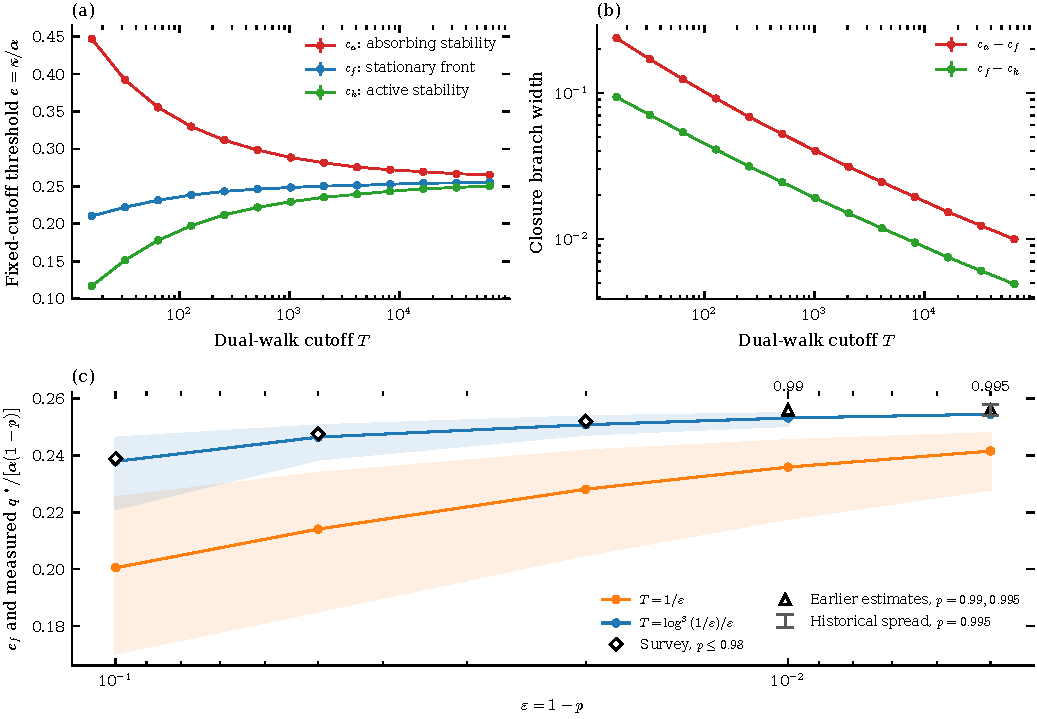
\includegraphics[width=\textwidth]{figs/fig_theory_v2}
\caption{Finite-time voter closure and cutoff sensitivity.
(a) Absorbing-state, stationary-front, and active-state thresholds of the
constant-diffusion closure at cutoff $T$. Bars are approximately 95\%
pointwise intervals from walk sampling.
(b) The two branches of the closure's bistable interval, with covariance
between thresholds retained.
(c) Matching prescriptions $T=1/\varepsilon$ and
$T=\log^3(1/\varepsilon)/\varepsilon$ compared with the finite-window
survey. Open triangles mark the earlier $p=0.99$ and 0.995 estimates.
The $p=0.995$ whisker is the historical spread
$q=0.000640\pm0.000005$, equivalent to $c=0.256\pm0.002$;
it represents estimator sensitivity. The longer $2\times10^7$-step runs
at that probability continue to decay. Shading varies either prescribed
time by a factor $A\in[1/4,4]$. The shading and historical whisker have
no assigned confidence coverage. Interpolation uses only recorded
cutoffs, leaving the upper logarithmic envelope incomplete at the
smallest $\varepsilon$.}
\label{fig:theory}
\end{figure*}

\subsection{Matching uncertainty and the voter endpoint}

In two dimensions the probability of retaining several distinct voter lineages
decays logarithmically with time~\cite{cox2010,cox2025}. The scale on which a
perturbation acts can therefore differ from $1/\varepsilon$ by logarithmic
factors. For example, the two-dimensional scaling of Ref.~\cite{cox2025}
uses $\varepsilon_N=(\log N)^3/N$. That result does not derive a matching
time for the present synchronous automaton, especially close to cancellation
of its leading cubic drift, but it motivates checking sensitivity to such
factors.

Figure~\ref{fig:theory}(c) compares the unadjusted prescriptions
$T=1/\varepsilon$ and $T=\log^3(1/\varepsilon)/\varepsilon$:
\begin{center}
\begin{tabular}{cccc}
$p$ & measured $c$ & $c_f(1/\varepsilon)$ & $c_f(\log^3(1/\varepsilon)/\varepsilon)$\\
\hline
0.9 & 0.2388 & 0.2005 & 0.2379\\
0.95 & 0.2476 & 0.2141 & 0.2464\\
0.98 & 0.2520 & 0.2281 & 0.2507\\
0.99 & 0.2560 & 0.2359 & 0.2531\\
0.995 & 0.2560 & 0.2415 & 0.2545
\end{tabular}
\end{center}
The logarithmic prescription substantially improves this comparison without
adjusting its prefactor. This comparison is sensitive to the matching scale, but does not validate
the prescription. In particular, the historical spread $5\times10^{-6}$ in
$q^*$ at $p=0.995$ corresponds to about $0.002$ in $c$, larger than the
theory--central-value difference at that point. That historical density
plateau subsequently decays (Fig.~\ref{fig:gpu_near20m}).
Multiplying either prescribed time by $A=1/4,1,4$ displays the remaining
sensitivity. Interpolation is linear in $\log T$; points beyond the recorded
range are left unevaluated.

The walk statistics constrain the closure much more precisely than they fix
its relation to the lattice process. For example, over $1024\le T\le65536$,
$c_f$ moves from $0.24843$ to $0.25526$, while its one-standard-error sampling
uncertainty grows from $0.00119$ to $0.00191$. We therefore do not assign a
confidence interval to a $T\to\infty$ amplitude. The same walks contribute
to successive checkpoint histograms; the stored marginal counts do not
recover their cross-time covariance, and we do not treat those checkpoints
as independent observations in an extrapolation.

The lazy-walk calculation gives another independent test of the closure.
At physical dual time $rT=65536$, it gives $c_f=0.2212$, $0.2060$, and
$0.2003$ for $r=1/2,1/4,1/8$, respectively, compared with measured values
about $0.218,0.216,0.219$. It captures the initial direction of the shift.
The measured differences among the smaller $r$ values lie below the
front-fit systematic variation discussed in Sec.~\ref{S-sec:async}, so this
comparison does not resolve a limiting amplitude. The five-cell rule in
Supplemental Sec.~\ref{S-app:molofsky} supplies a sharper limitation: no single cutoff describes its early seed-growth crossover, observed bulk
stationarity range, and extrapolated onset of coherent expansion.

The exact identities identify a mechanism available to a voter perturbation:
higher-lineage correlations generate the noncubic drift needed for a bistable
reaction term. They also explain why that contribution becomes small at long
voter times within the closure. Whether it remains effective after matching
and fluctuation corrections is not determined by the calculation. Persistence
of a first-order line for every fixed $p<1$, and its logarithmic approach to
the voter point, remain conjectures; the numerical evidence for finite $p$
is assessed separately in Sec.~\ref{sec:voter}.


\section{Discussion}
\label{sec:discussion}

At $p=\alpha=1/2$ the numerical evidence supports a discontinuous
active--absorbing transition in a two-dimensional binary rule with
exactly two absorbing configurations. The central observation is
finite, spatially distributed and dynamically sustained activity
across the measured front-reversal region. Prepared fronts reverse
direction while retaining an active interior; bulk decay on the
lower-$q$ side proceeds through absorbing-domain growth; disks and holes
exchange their growth signs on opposite flanks.
The directional crossing differences and their window dependence
limit the resolution of a unique boundary, but do not remove this
combined evidence for phase competition.

The novelty is this joint quantitative test of activity and invasion.
Earlier work reported discontinuous two-state behavior~\cite{rodrigues2015},
and ecological alliance models exhibit related fronts and active
layers~\cite{szabo2004,guisoni2013}. The binary construction isolates
the phenomenon from internal dynamics of an absorbing alliance.
It also distinguishes a discontinuous loss of local activity from
the magnetization jump at a GV transition.

The finite-time closure identifies a specific microscopic contribution:
five or more ancestral lineages generate the noncubic reaction terms
needed for bistability. Its exact identities concern the unperturbed
voter law at a prescribed cutoff. Matching that law to the stochastic
lattice process in two dimensions, especially near cancellation of the
leading drift, remains an approximation. The five-cell comparison
makes the distinction concrete (Supplemental Sec.~\ref{S-app:molofsky}):
a one-sided extrapolation locates the onset of coherent expansion,
but interior decay prevents resolving coherent retreat with a persistent
active interior.
Early seed growth, finite-window bulk stationarity and linear stability
are different quantities.

A predictive spatial theory would need to account for front motion,
curvature and the nucleation rate as well as local drift.
For wetting, it would also need the interaction between the two active
fronts bounding a film. The measured adsorption increase does not fix
that interaction or an asymptotic exponent.
Finally, the near-voter measurements demonstrate why agreement across
sizes at one horizon is insufficient to establish stationarity.
Whether the discontinuity persists for every fixed $p<1$, or ends
before the voter point, is not determined here.


\begin{acknowledgments}
Simulations were run on the Torch cluster at New York University.
\end{acknowledgments}

\section*{Data availability}
The accompanying manuscript-source archive contains this paper, its supplement,
and the exact figure files. A separate reproducibility archive contains the
CPU and CUDA source code, parameter and seed manifests, reduced tables,
analysis and figure scripts, and a documented rebuild procedure.
The companion input-data archive provides the locally available trajectories,
profiles, final configurations, and legacy figure reductions used by those
analyses. Per-file checksums and explicit provenance distinguish raw inputs,
retained reductions, and the new analyses. The original snapshots underlying
the removed free-band roughness comparison are unavailable locally; the
revised wall plot uses the archived wall-edge reductions. No public repository
identifier is assigned in this review draft.

\bibliography{refs}
\end{document}
